\input{../header}
\rhead{Your name: \rule{8cm}{0.15mm}}

\begin{document}
%
\section{Learning target DF0, version 1}
Compute and interpret average velocity and its units, using information about the position function (as a table, graph, and/or function formula).

\hrulefill

The position (in miles), $s(t)$, of a car driving along a straight road at time $t$ (in minutes), is given by the following graph. \\
		
	%	\begin{center}
		\scalebox{0.35}{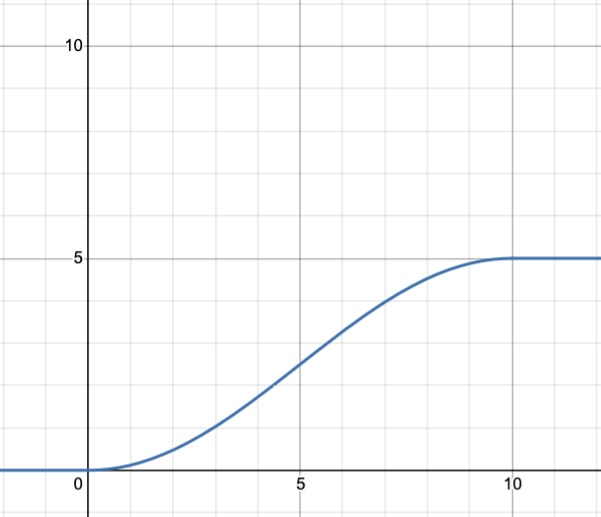
\includegraphics{../images/LT1-1-S24.jpg}}
	%	\end{center}
		
\begin{enumerate}
	\item Determine the average velocity of the car between $t=5$ and $t=10$ minutes, $AV_{[5,10]}$. Use proper notation and the work you did to determine the result; include units on your answer.

	\vspace{1in}

	\item On the graph of $s(t)$ draw a line through  $(3,s(3))$ and $(7,s(7))$; what is the slope of this line and what does that slope mean in the physical context of the function $s$?  
	
	\vspace{0.85in}
	
	
	\item Here's some additional data for the function $s(t)$ that's pictured above: 
	
	\begin{center}
		\begin{tabular}{|c|c|c|c|c|}
			\hline
			$t$ (in minutes) & 8.0 & 8.05 & 8.1 & 8.15 \\
			\hline
			$s(t)$ (in miles) & 4.52254 & 4.54537 & 4.56770 & 4.58952\\
			\hline
		\end{tabular}
	\end{center} 
	
	Find the average velocity of the car on the interval $[8.05, 8.1]$. Label your result using proper notation and include units on your answer.
	
\end{enumerate}
%%%%%%%%%%%%%%%%%%%%%%%%%%%%%%%%%%%%%%%%%%%%%%%%%%%%%%%%%
\pagebreak
%%%%%%%%%%%%%%%%%%%%%%%%%%%%%%%%%%%%%%%%%%%%%%%%%%%%%%%%%

\section{Learning target DF0, version 2}
Compute and interpret average velocity and its units, using information about the position function (as a table, graph, and/or function formula).

\hrulefill
\begin{enumerate}[leftmargin=10pt]

	\item Your fitbit records some data about the distance you traveled on a bike ride around the city:
	
	\begin{center}
		\begin{tabular}{|c|c|c|c|c|c|c|}
		\hline
		$t$ (in minutes) & 0 & 15 & 30 & 45 & 60 & 75 \\
		\hline
		$d(t)$ (in miles) & 0 & 4.5 & 10.5 & 15 & 21 & 24\\
		\hline
		\end{tabular}
		\end{center}
	Find your average velocity over the time interval from $t = 30$ to $t = 75$. Include units.
	
	\vfill

	\item The following graph shows a plot of the function $s(t)$ that measures the location of a car (in thousands of feet) along a road at time $t$ in minutes.
	
	\begin{center}
	\scalebox{0.65}{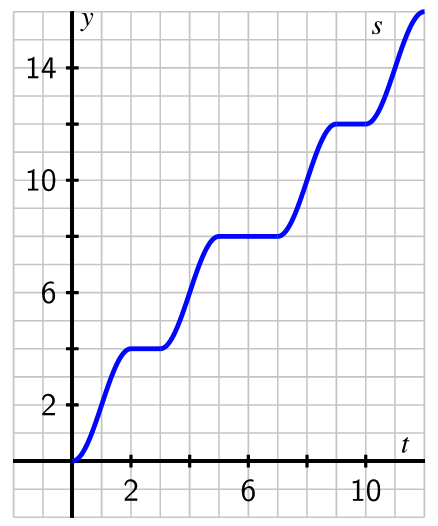
\includegraphics{../images/CP-3-01-s.png}}
	\end{center}
		
	\begin{itemize}
		\item Use the graph to find the average velocity of the car between $t=2$ and $t=7$ minutes, $AV_{[2,7]}$. Include units on your answer.
		
		
		\vfill

		\item On the graph of $s(t)$ draw a line through $(7,s(7))$ and $(10,s(10))$; what is the slope of this line, and what does that slope mean in the physical context of the function $s$?  Include units on your answer.
		
		
	\end{itemize}

\end{enumerate}
\end{document}